\section{Work done in a reversible process:Ideal gas  systems}
The main concern of the study of thermodynamics is the efficient extraction of useful work.Work can be extracted mainly in two ways,reversible and irreversible.A process,which can be retraced along the same path is called a reversible process.In this path,all the system properties are well defined and hence the work done ,W can be written as

\begin{equation}
	W=\int_{V_1}^{V_2}{PdV}
	\label{eqn:revwork}
\end{equation}
\begin{center}
Reversible work done ~\cite{fleming_me027}
\end{center}
where $V_1$ and $V_2$ are initial and final volumes and P,the instantaneous pressure of gas.

\subsection{Isothermal expansion}
\begin{figure}[h]
	\begin{center}
		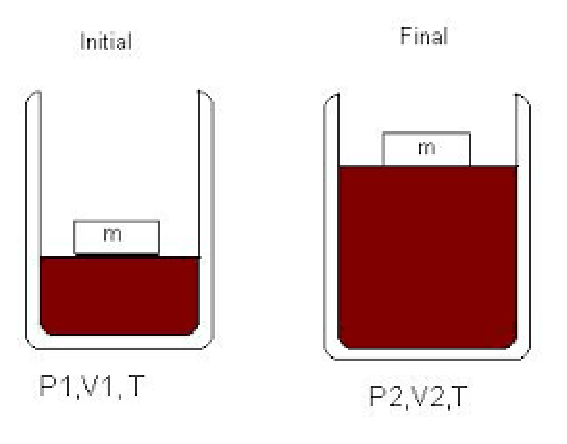
\includegraphics[width=200px]{me20b027a.eps}
	\end{center}
	\caption{Reversible Isothermal Expansion~\cite{libtex_me027}}
	\label{fig:revexp}
\end{figure}
The workdone in an isothermal process can be generalised from equation~\ref{eqn:revwork} as following
$$W=\int_{V_1}^{V_2}{PdV}$$
$$P=\frac{nRT}{V}$$
$$W=nRT\int_{V_1}^{V_2}{\left(\frac{dV}{V}\right)}$$
\begin{equation}
	W=nRT\ln\left(\frac{V_2}{V_1}\right)
\end{equation}
\\\\\\
The figure~\ref{gr:istexp} below,depicts the isothermal expansion of the ideal gas with area under the graph as the workdone

\begin{figure}[h]
	\begin{center}
		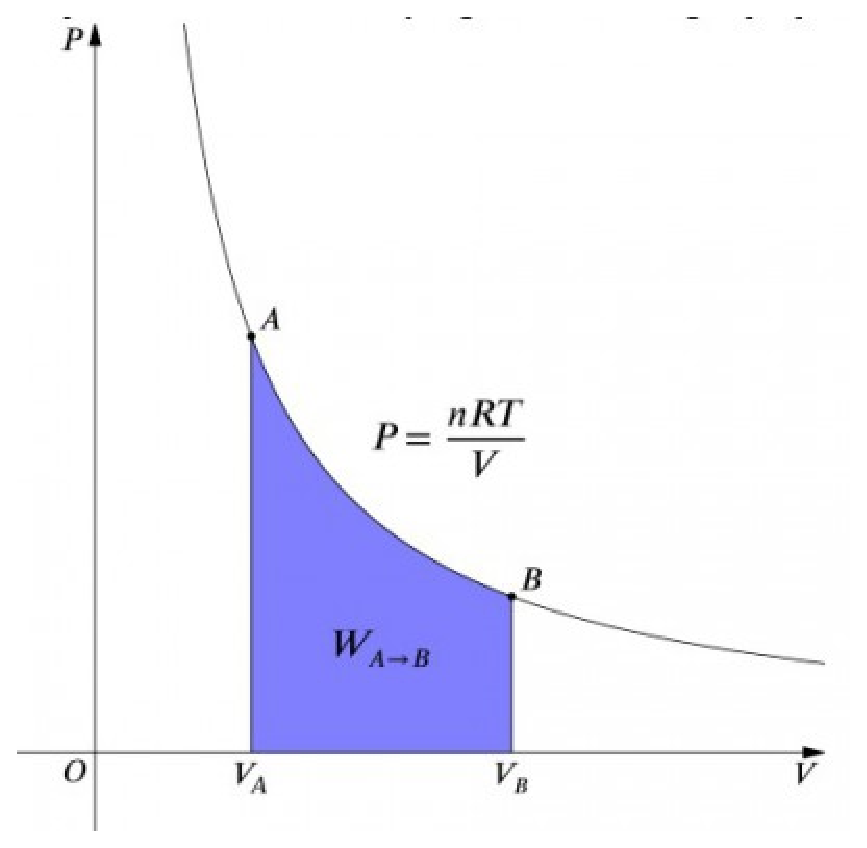
\includegraphics[width=200px]{me20b027b.eps}
	\end{center}
	\caption{P-V diagram for isothermal expansion~\cite{donev_me027}}
	\label{gr:istexp}
\end{figure}
